\chapter{Monte Carlo simulations of designs}
\label{chapter:optimization}
\label{c6:monte-carlo}
In this chapter, Monte Carlo simulations of the six unoptimized instrument design variants introduced in Chapter \ref{c3} will be presented. Simulations are performed using McStas \cite{willendrup2020} with instrument files derivative of \texttt{SEMSANS\_Delft} \cite{bouwman2021b}. The goal is to complement the analysis and constraints discussed in Chapter $\ref{c4:constraints}$ and provide an understanding of how instruments might behave in practice for samples representative of the target range of $\SI{10}{\nano\meter}$ to $\SI{5}{\micro\meter}$. Additionally, two ways in which (simulated) measurement data can be analyzed will be discussed. 
\section{Simulated measurements}
Although simple mathematical models such as those used in Section \ref{c4.4} can give a first understanding of single scattering by making many assumptions, such methods are inadequate when considering the full complexity of multiple scattering, polychromatic beams, divergence, etc. These factors come into play when performing real SEMSANS measurements. Simulating such measurements requires Monte Carlo methods, which rely on the principle that simulating realistic behavior of a large number of neutrons $N$ can give an estimate of quantities like detector intensity with uncertainty proportional to $1/\sqrt{N}$.  

To test the ability of the six unoptimized instruments introduced in Chapter \ref{c3} to measure samples in the target range, a series of such Monte Carlo simulations is performed. Measurements are simulated for samples of the type described in Sections \ref{c2.4}, \ref{c3.5} with radii $R = \SI{50}{\nano\meter}, \SI{300}{\nano\meter}, \SI{2}{\micro\meter}$. Although these could in principle all be simulated with other sample parameters like sample thickness $t$ the same, this would cause the scattering power $\tau$ as defined in Equation \eqref{eq:sample-tau} to vary greatly and cause it to go too far out of the range of $0.1$ and $0.8$ that is typically considered to be optimal in terms of signal-to-noise ratio \cite{bouwman2021b}\cite{heijkamp2011}. For this reason, $t$ is varied between $1 - 10 ~\unit{\milli\meter}$ for different $\lambda_0, R$ pairings to optimize $\tau$. The remaining sample parameters take values $\phi = 0.015$, $\Delta\rho = \SI{1.8e10}{\centi\meter}^{-2}$ and are the same in each case. The chosen $t$ values with the corresponding $\tau$ are shown in Table \ref{tab:sample-thickness}.

\begin{table}[h!]
	\centering
	\begin{tabular}{cc|cc}
		\toprule
		$\lambda_0~[\unit{\angstrom}]$  & $R ~[\unit{\nano\meter}]$  & $t ~[\unit{\milli\meter}]$& $\tau~[\unit{\meter^3}]$ \\
		\midrule
		\num{4.321} & \num{50} & \num{10} & \num{0.067}\\
		\num{4.321} & \num{300} & \num{10} & \num{0.4022} \\
		\num{4.321} & \num{2000} & \num{1} & \num{0.2681} \\
		\num{8} & \num{50} & \num{10} & \num{0.2298} \\
		\num{8} & \num{300} & \num{5} & \num{0.6893} \\
		\num{8} & \num{2000} & \num{1} & \num{0.9191} \\
		\bottomrule
	\end{tabular}
	\caption{Combinations of $\lambda_0$ and sample radius $R$ with a sample thickness $t$ chosen to keep $\tau$ approximately within the optimal range of $0.1$ and $0.8$.}
	\label{tab:sample-thickness}
\end{table}

\subsection{Measurement procedure}
For each of the six instruments, measurements on the three samples with radii and thicknesses as given in Table \ref{tab:sample-thickness} were simulated. Additionally, empty measurements were simulated in each case to establish a baseline for visibility. 

To perform a measurement, a range of $B$-field strength values is simulated with the analyzer in the $+x$ and $-x$ settings. This is done with and without a sample, resulting in four separate simulations for each data point. Although in principle the full range of $B$-values bounded by the focussing condition could be simulated, only $B$-values were considered that correspond to the respective instrument $\delta$-range as given in Table \ref{tab:designs-final-ranges} in Chapter \ref{c4:constraints}. The sample range was $\frac{R}{10} - 3R$ and the overlap between each instrument range and these sample ranges was computed. In each case there was overlap, and 30 $B$-settings corresponding to the overlapping $\delta$-range were chosen. $B$-resolution limitations were not considered here but can in practice be expected to limit the number of practical measurements to fewer than 30. It should be noted that $\delta$ is computed from $\lambda_0$ so that $\delta = \lambda_0^2L_s\alpha$. This will have consequences for the measured signal as indicated in Section \ref{c3.6}.

\subsection{Simulation setup}
To simulate the instruments, version 3.4 of the raytracing software package McStas \cite{willendrup2020} is used with OpenACC acceleration enabled. The simulations were performed on a desktop computer with an Intel Core i5-6600 quad-core 3.3 GHz CPU and an Nvidia GeForce GTX 1060 GPU. Simulated instruments are all derivative of the previously simulated \texttt{SEMSANS\_Delft} instrument \cite{bouwman2021b}. The \texttt{Foil\_flipper\_magnet} component was used to simulate foil flippers like in \texttt{SEMSANS\_Delft} and idealized components for the Wollaston prism and isosceles triangle were derived from the existing \texttt{Pol\_triafield} component. Each $B$-field and analyzer setting was simulated using $10^7$ neutrons when using foil flippers and $10^8$ when using prisms or triangles. This is due to the large difference in simulation time. Simulation time for a single simulation of $10^6$ varied from well under $\SI{1}{\second}$ for the prisms and triangles to about $\SI{4}{\second}$ for the foil flippers, presumably due to the greater complexity of the corresponding McStas component. 
The \texttt{SANS\_spheres2} sample component is used to model the described sample. Although most of its parameters correspond directly to those listed above, two that deserve mention are \texttt{Qmind} and \texttt{Qmaxd} which define the simulated $Q$-range. As the sample $R$ values span almost two orders of magnitude, the corresponding $Q$ range is quite different for the three samples and is proportional to $1/R$. This is accounted for by using \texttt{Qmind}$=0.1/R$, \texttt{Qmaxd}$=10/R$, matching the sample $Q$-range as discussed in Section \ref{c2.4}.

\subsection{Data analysis}
To estimate $P(\delta) = e^{G(\delta)  - \tau}$, two analysis methods are used to compute an estimate $P_{exp}(\delta)$ from the simulation data. The first is based on fitting an expected modulation pattern as done elsewhere \cite{bouwman2011}\cite{parnell2023}, and the second uses RMS values. The advantage of the second method is that it is more robust and better suited for real measurement conditions where many factors such as beam characteristics shape the observed modulation profile. Both rely on computing the modulation visibility $V(y)$, defined as 
$$V(y) = \frac{I_{up}(y) - I_{down}(y)}{I_{up}(y) + I_{down}(y)}$$
Here $I_{up}, I_{down}$ correspond to simulated measurements using the $\pm x$ analyzer settings. Intuitively, this gives a normalized expression for the modulation amplitude, allowing for some variation in total measured intensity $I_{up}(y) + I_{down}(y)$ across the detector. The signal at the boundaries of the detector is still not useful due to effects such as discussed in Section \ref{c4.4} and only the middle $\SI{6}{\milli\meter}$ is used when estimating $P(\delta)$ for this reason.

In the first method, a modulation pattern with a Gaussian envelope similar to Equation \eqref{eq:poly-base-modulation} is fitted with variable amplitude to $V(y)$. Because $V(y)$ is used, $I_0$ disappears from the expression and $V_{b,s}(y)$ can largely be described by just $V_{\text{gauss}}(y) = A_{b,s}E(y)\cos(2\pi\alpha\lambda_0y)$ with fitted amplitudes $A_{b,s}$. In practice, a small error term $\epsilon$ is included to compensate for a potential non-zero average. This gives the final fitting function with parameters $A_{b,s}, \epsilon$
\begin{equation}
	V_{\text{fit}}(y) = \epsilon+ A_{b,s}E(y)\cos(2\pi\alpha\lambda_0y) \label{eq:gauss-fit-function}
\end{equation}
The resulting amplitudes $A_b, A_s$ with and without a sample at a given $B$ (and $\delta$) setting are then related to $P(\delta)$ via $P_{exp}(\delta) = A_s/A_b$. 

In the second method, the RMS of $V(y)$ is computed as $RMS_{b,s}$ and again $P_{exp}(\delta)$ is given by the ratio $P_{exp}(\delta) = RMS_s/RMS_b$.

\section{Results}
The result of the described simulation and data analysis using both methods is shown in Figures \ref{fig:simulation-plot-gauss}, \ref{fig:simulation-plot-rms}, with each subfigure showing simulated measurements within the accessible $\delta$-ranges for each design together with computed $P_{exp}(\delta)$ and analytical $P(\delta)$. Additionally, Figure \ref{fig:simulation-raw-intensity} shows an example of how raw simulation data from a simulated measurement using WP 8 is processed and fitted to $P_{exp}(\delta)$ in the two ways. The corresponding values are $P_{exp} = 0.5219 \pm 2 \cdot 10^{-4}$ when using the Gauss method and $P_{exp} = 0.5219 \pm 3 \cdot 10^{-4}$ when using the RMS. The analytical value is $P(\delta) = 0.501906$, which is incompatible with both estimates and their standard error. These values were computed from fitted amplitudes $A_b = 0.999905 \pm 8\cdot 10^{-6}$, $A_s = 0.5218 \pm 2 \cdot 10^{-4}$ and RMS values $RMS_b = 0.66674 \pm 6\cdot 10^{-5}$ and $RMS_s = 0.3479 \pm 2 \cdot 10^{-4}$. In both cases, the uncertainty with a sample is much greater than without.
\begin{figure}[htbp]
	\centering
	\begin{subfigure}[b]{0.45\textwidth}
		\centering
		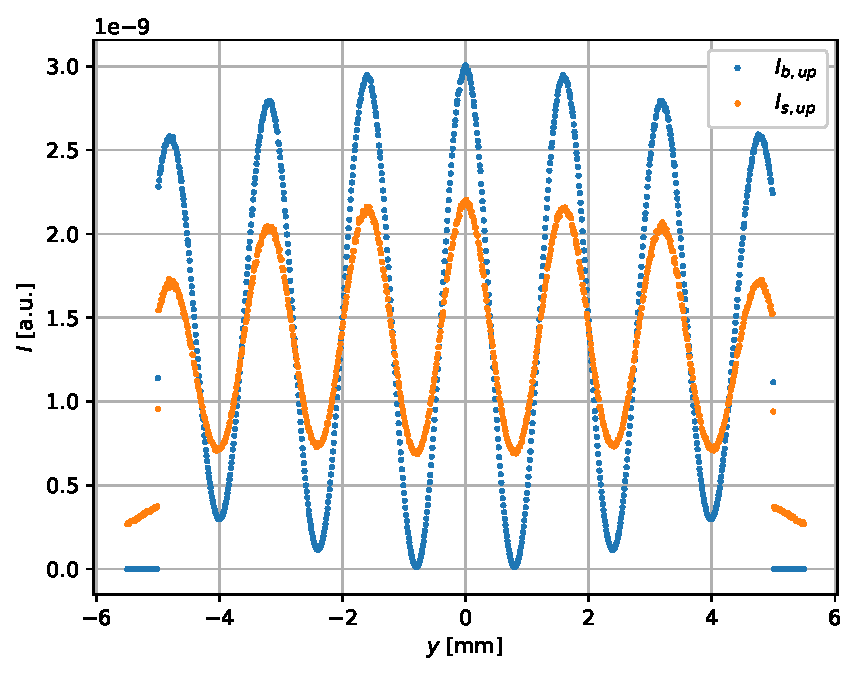
\includegraphics[width=\textwidth]{simulation-raw-intensity-up}
		\caption{$I_{b,up}$ and $I_{s,up}$.}
		\label{fig:simulation-raw-intensity-up}
	\end{subfigure}
	\hfill
	\begin{subfigure}[b]{0.45\textwidth}
		\centering
		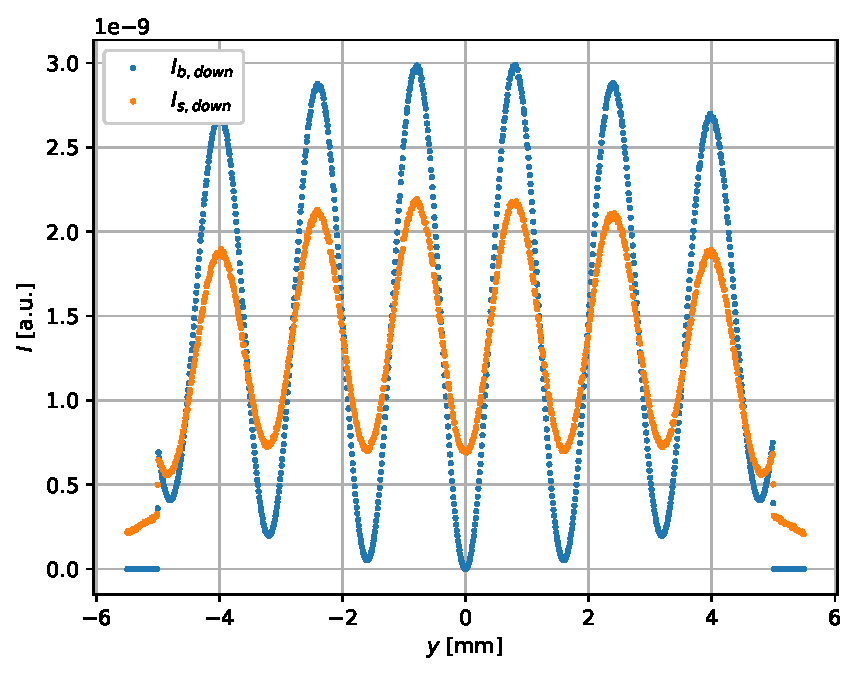
\includegraphics[width=\textwidth]{simulation-raw-intensity-down}
		\caption{$I_{b,down}$ and $I_{s,down}$.}
		\label{fig:simulation-raw-intensity-down}
	\end{subfigure}
	\centering
	\begin{subfigure}[b]{0.45\textwidth}
		\centering
		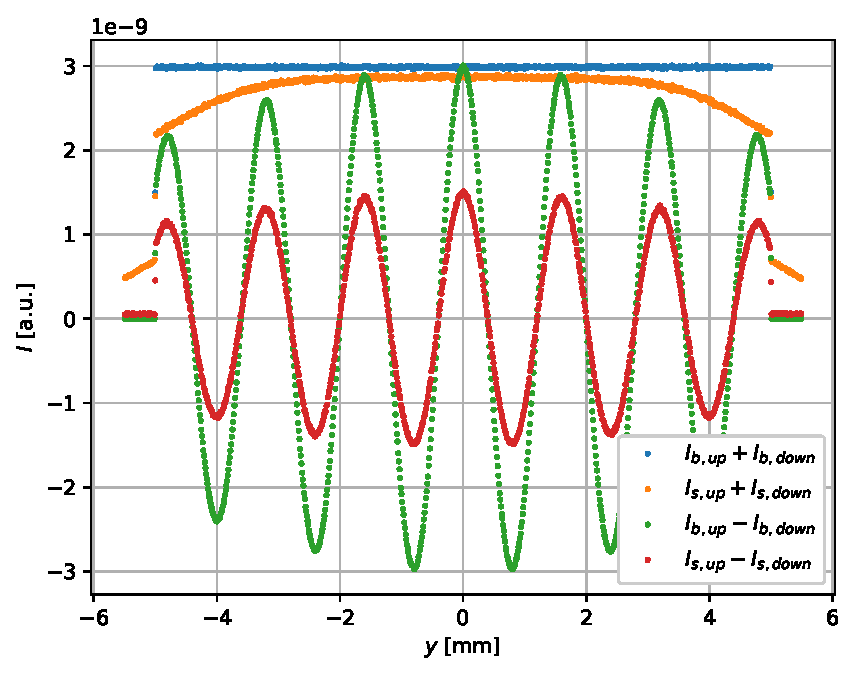
\includegraphics[width=\textwidth]{simulation-raw-intensity-differential}
		\caption{$I_{b,up} \pm I_{b,down}$ and $I_{s,up} \pm I_{s,down}$.}
		\label{fig:simulation-raw-intensity-differential}
	\end{subfigure}
	\hfill
	\begin{subfigure}[b]{0.45\textwidth}
		\centering
		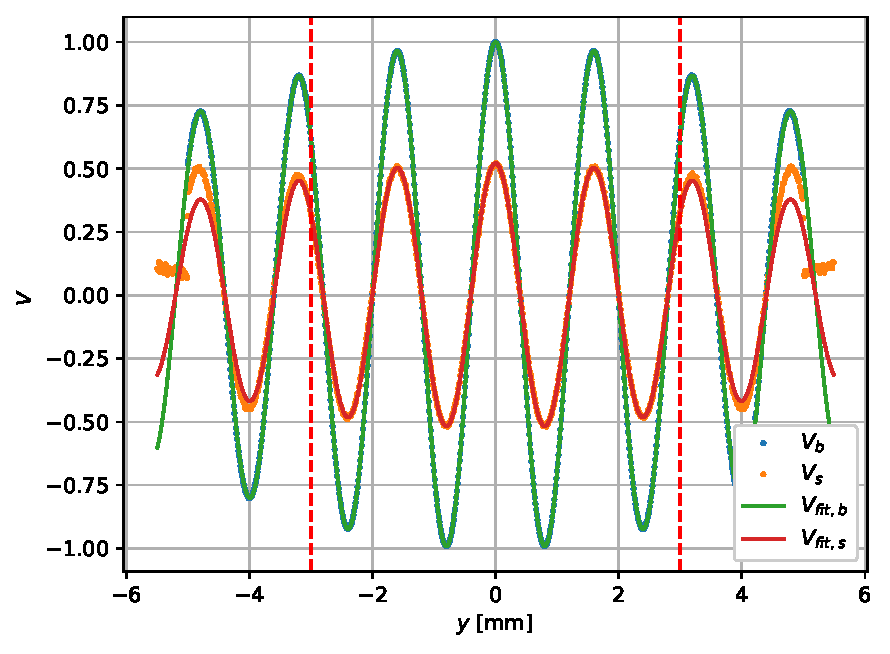
\includegraphics[width=\textwidth]{simulation-raw-intensity-pol}
		\caption{$V_b, V_s$ and fitted Gaussian modulations $V_{fit,b}, V_{fit,s}$.}
		\label{fig:simulation-raw-intensity-pol}
	\end{subfigure}
	\caption{An illustration of the detector intensity patterns recorded during simulations and how they are processed to a fit. The data corresponds to a simulated measurement using WP 8 of the $R = \SI{300}{\nano\meter}$ sample with $B_1 = \SI{5.4}{\milli\tesla}, B_2 = \SI{10.8}{\milli\tesla}$, corresponding to $\delta = \SI{900}{\nano\meter}$. The fit values are shown in Figure \ref{fig:simulation-plot-gauss-WSP-8} and \ref{fig:simulation-plot-rms-WSP-8}. Figure \ref{fig:simulation-raw-intensity-up}, \ref{fig:simulation-raw-intensity-down} show the detector intensities overlaid with and without sample for both analyzer settings (up and down). From these, signals are derived by adding and subtracting the up and down intensities. Finally, $V(y)$ is computed and from the $V(y)$ values in the middle $\SI{6}{\milli\meter}$ of the detector $P_{exp}(\delta)$ is computed by fitting modulation patterns with a Gaussian envelope or by computing the RMS.}
	\label{fig:simulation-raw-intensity}
\end{figure}

\begin{figure}[p]
	\centering
	\begin{subfigure}[b]{0.45\textwidth}
		\centering
		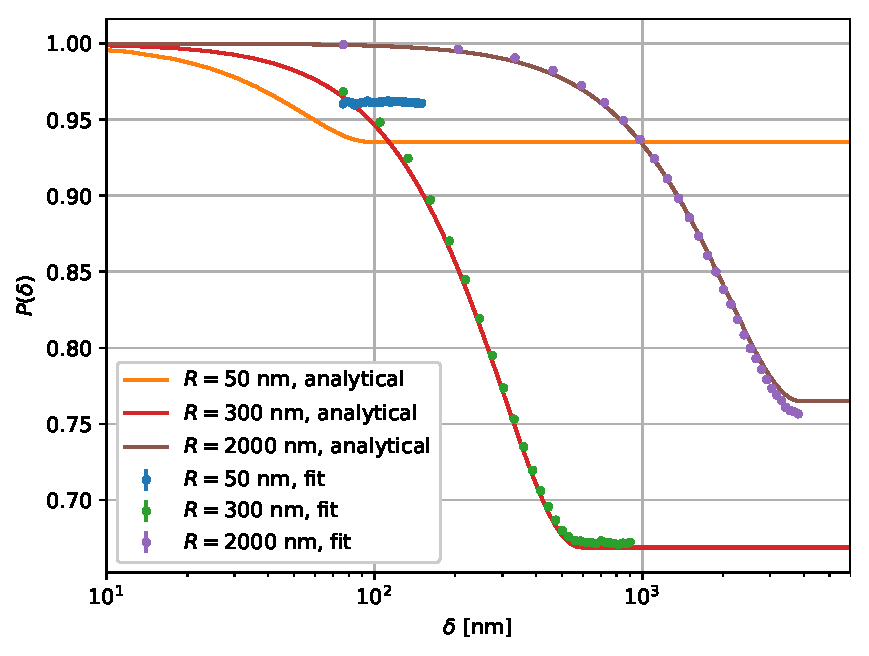
\includegraphics[width=\textwidth]{simulation-plot-gauss-FOIL-4.321}
		\caption{FOIL 4.321.}
		\label{fig:simulation-plot-gauss-FOIL-4.321}
	\end{subfigure}
	\hfill
	\begin{subfigure}[b]{0.45\textwidth}
		\centering
		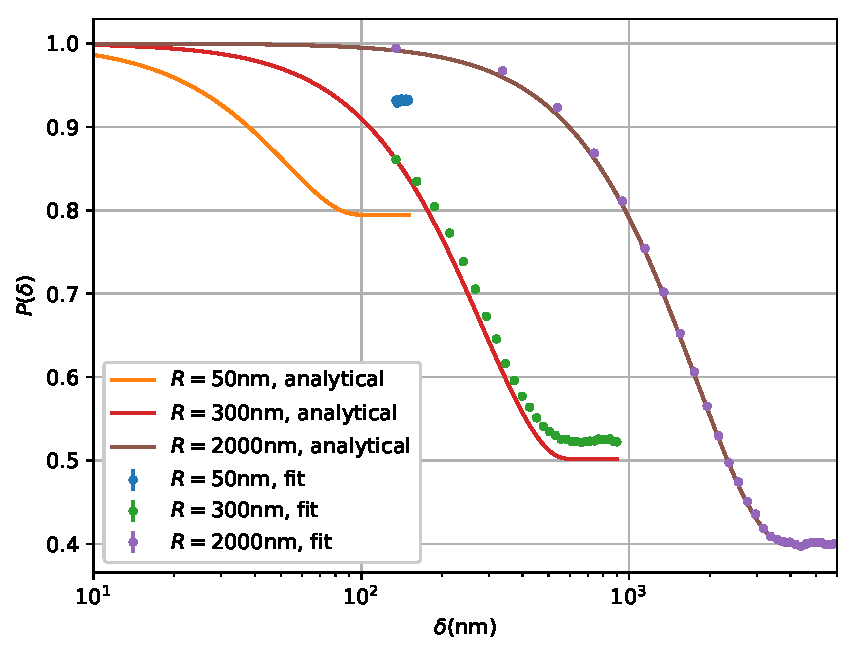
\includegraphics[width=\textwidth]{simulation-plot-gauss-FOIL-8}
		\caption{FOIL 8.}
		\label{fig:simulation-plot-gauss-FOIL-8}
	\end{subfigure}
	\centering
	\begin{subfigure}[b]{0.45\textwidth}
		\centering
		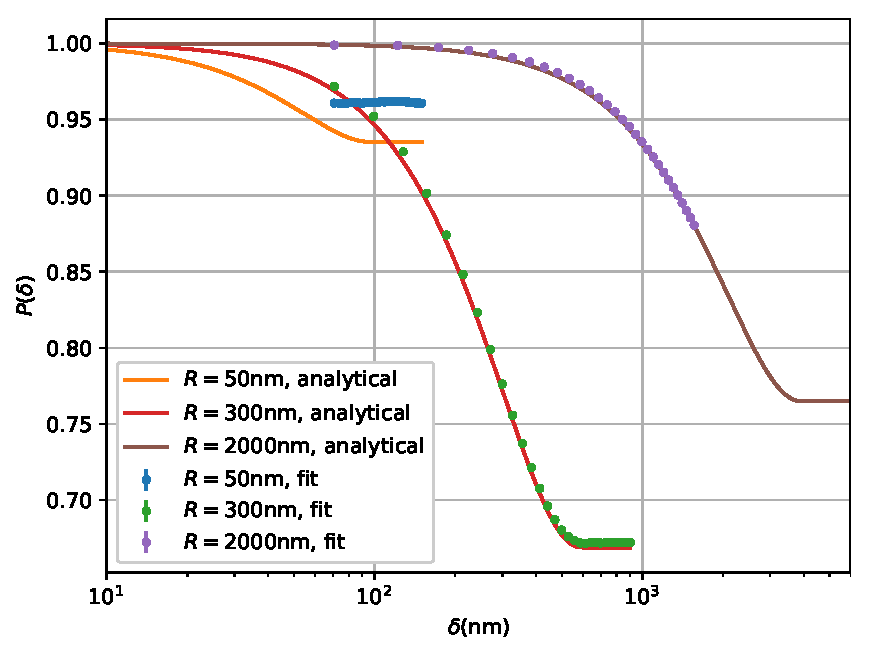
\includegraphics[width=\textwidth]{simulation-plot-gauss-WSP-4.321}
		\caption{WP 4.321.}
		\label{fig:simulation-plot-gauss-WSP-4.321}
	\end{subfigure}
	\hfill
	\begin{subfigure}[b]{0.45\textwidth}
		\centering
		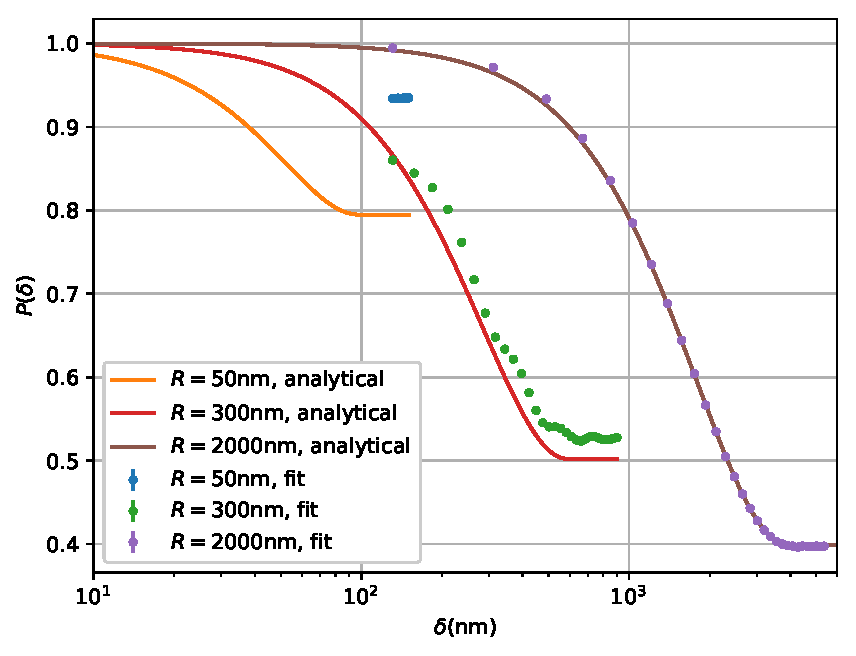
\includegraphics[width=\textwidth]{simulation-plot-gauss-WSP-8}
		\caption{WP 8.}
		\label{fig:simulation-plot-gauss-WSP-8}
	\end{subfigure}
	\centering
	\begin{subfigure}[b]{0.45\textwidth}
		\centering
		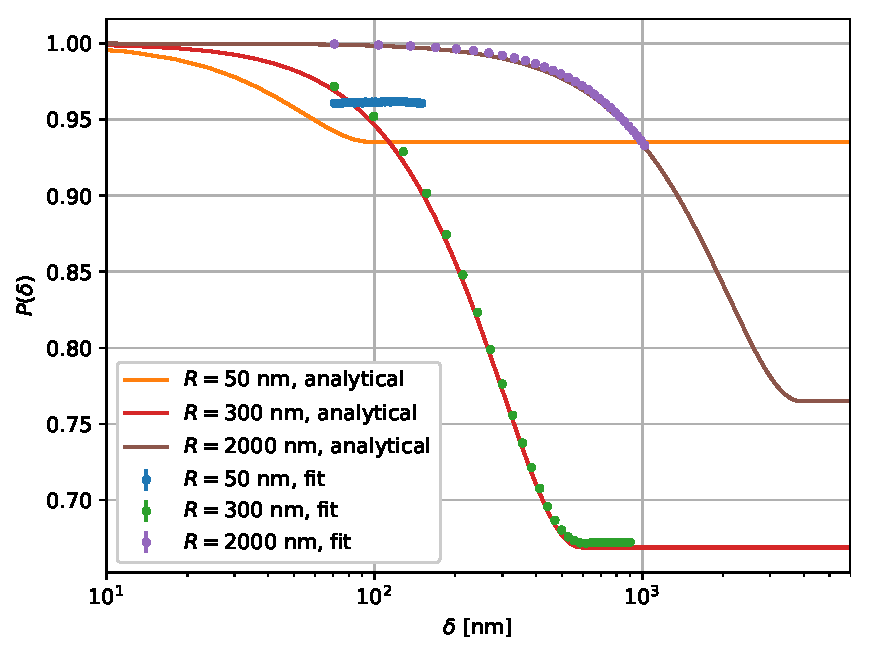
\includegraphics[width=\textwidth]{simulation-plot-gauss-ISO-4.321}
		\caption{ISO 4.321.}
		\label{fig:simulation-plot-gauss-ISO-4.321}
	\end{subfigure}
	\hfill
	\begin{subfigure}[b]{0.45\textwidth}
		\centering
		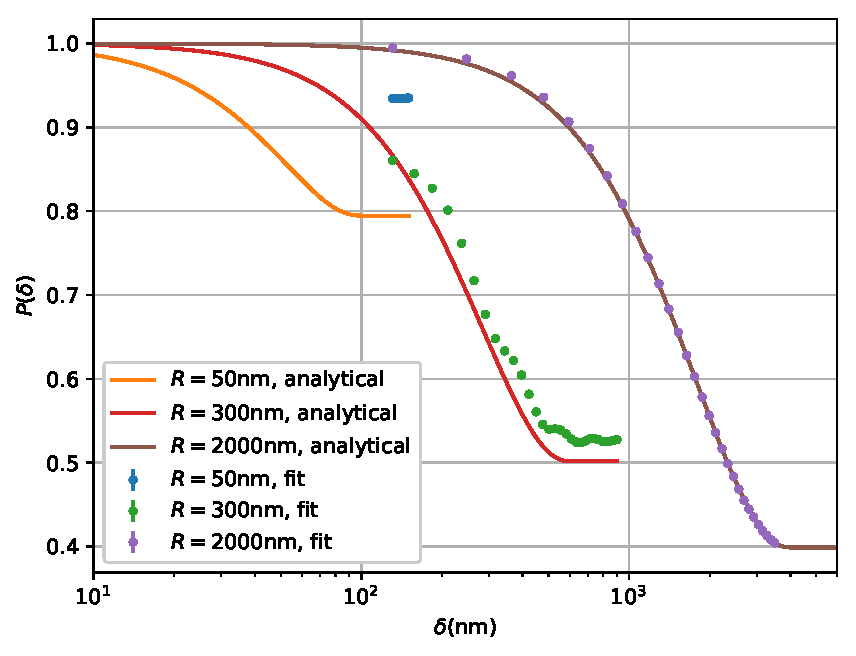
\includegraphics[width=\textwidth]{simulation-plot-gauss-ISO-8}
		\caption{ISO 8.}
		\label{fig:simulation-plot-gauss-ISO-8}
	\end{subfigure}
	\caption{$P_{exp}(\delta)$ values derived from a fit of a Gaussian modulation envelope to detector intensity simulation data. Measurements using each of the six instruments were simulated using three samples as specified in Table \ref{tab:sample-thickness} together with the corresponding analytical $P(\delta)$. The error bars are too small to be seen.}
	\label{fig:simulation-plot-gauss}
\end{figure}

\begin{figure}[p]
	\centering
	\begin{subfigure}[b]{0.45\textwidth}
		\centering
		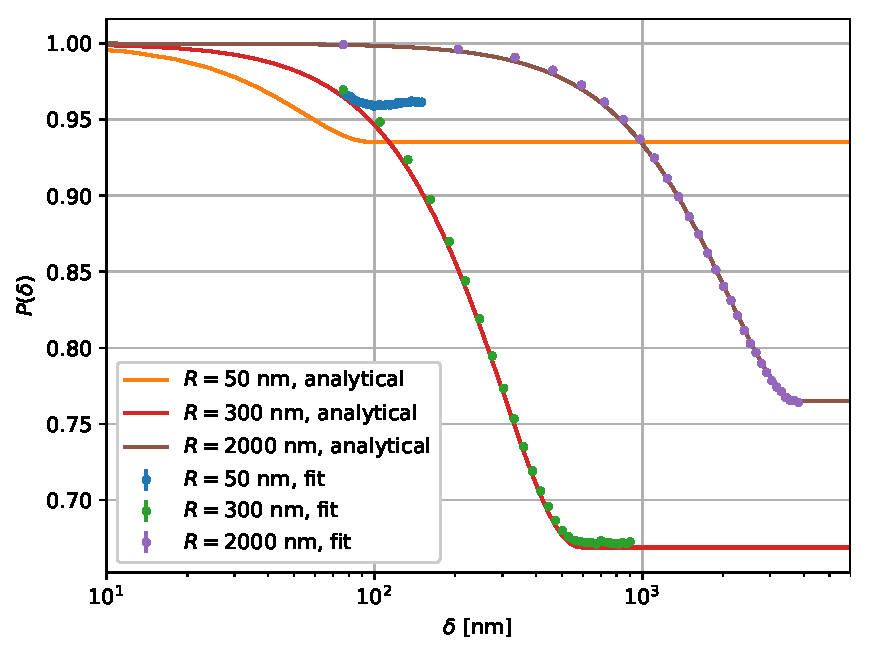
\includegraphics[width=\textwidth]{simulation-plot-rms-FOIL-4.321}
		\caption{FOIL 4.321.}
		\label{fig:simulation-plot-rms-FOIL-4.321}
	\end{subfigure}
	\hfill
	\begin{subfigure}[b]{0.45\textwidth}
		\centering
		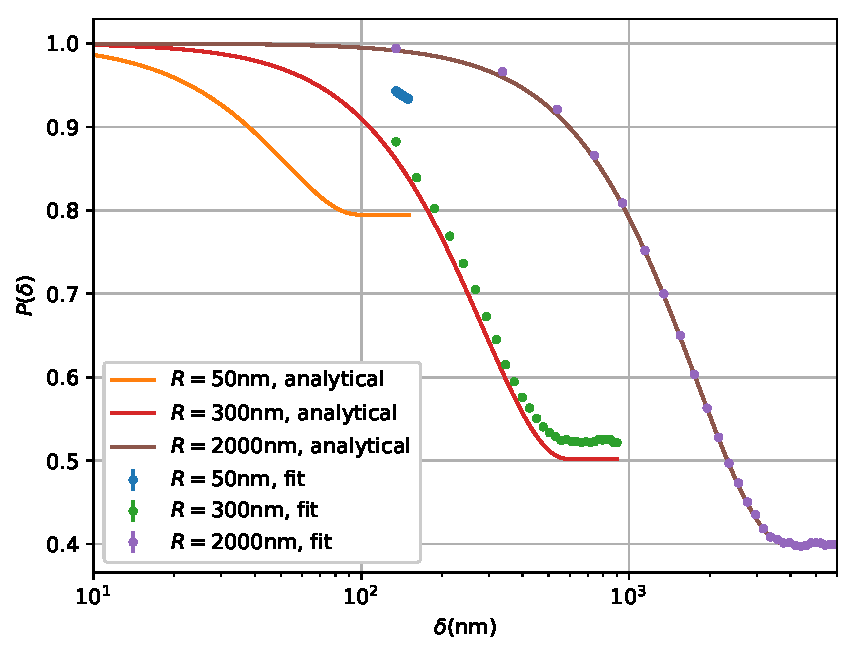
\includegraphics[width=\textwidth]{simulation-plot-rms-FOIL-8}
		\caption{FOIL 8.}
		\label{fig:simulation-plot-rms-FOIL-8}
	\end{subfigure}
	\centering
	\begin{subfigure}[b]{0.45\textwidth}
		\centering
		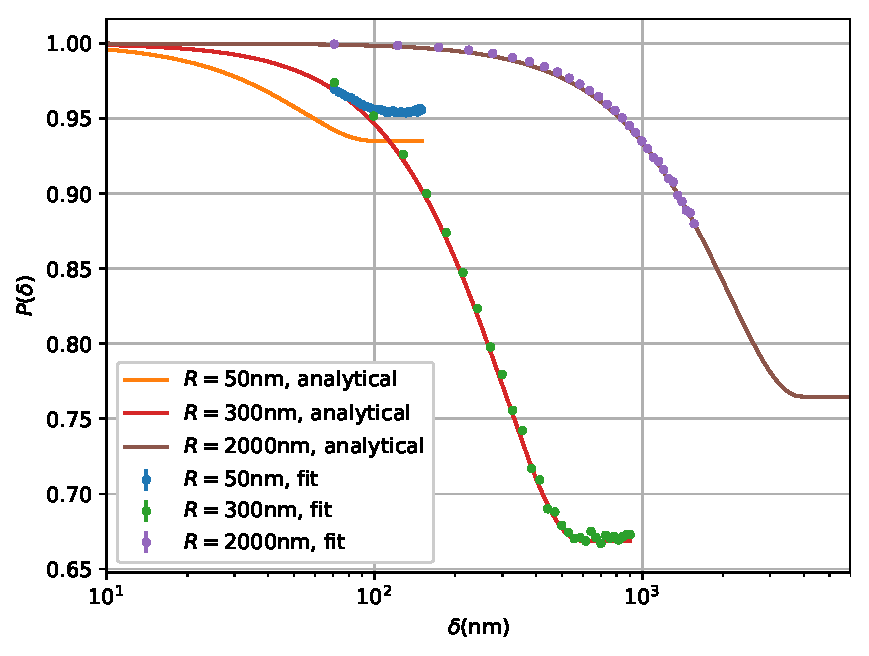
\includegraphics[width=\textwidth]{simulation-plot-rms-WSP-4.321}
		\caption{WP 4.321.}
		\label{fig:simulation-plot-rms-WSP-4.321}
	\end{subfigure}
	\hfill
	\begin{subfigure}[b]{0.45\textwidth}
		\centering
		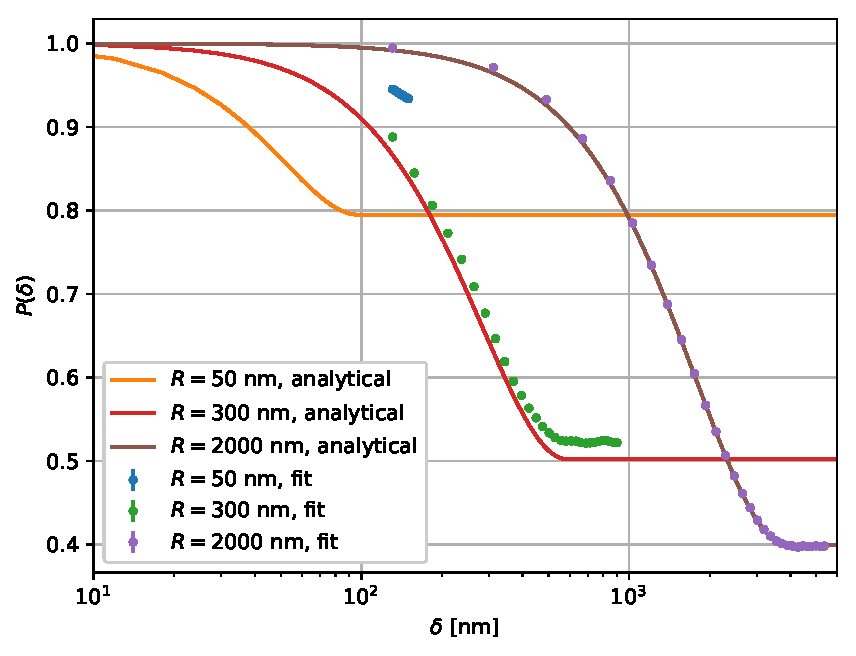
\includegraphics[width=\textwidth]{simulation-plot-rms-WSP-8}
		\caption{WP 8.}
		\label{fig:simulation-plot-rms-WSP-8}
	\end{subfigure}
	\centering
	\begin{subfigure}[b]{0.45\textwidth}
		\centering
		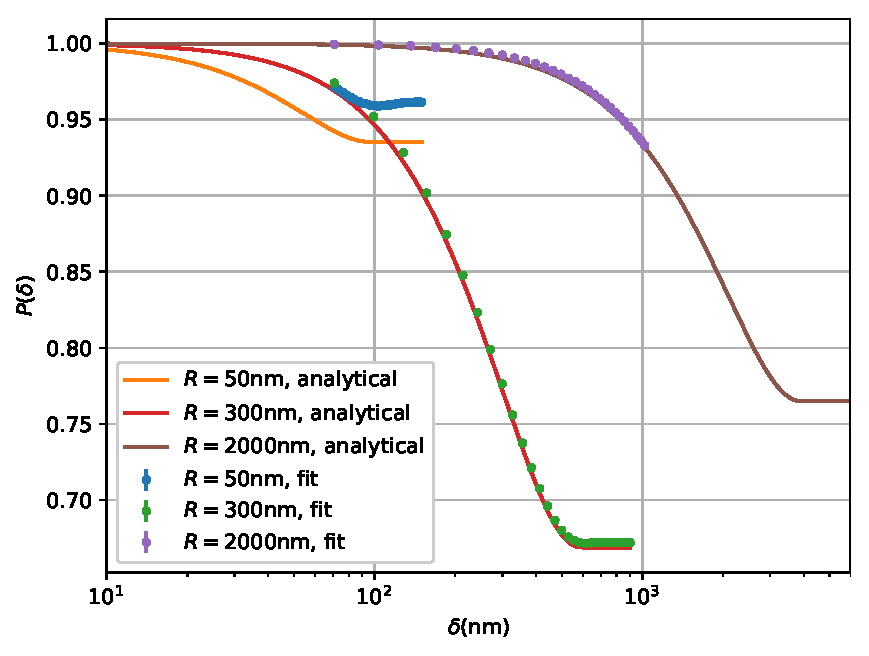
\includegraphics[width=\textwidth]{simulation-plot-rms-ISO-4.321}
		\caption{ISO 4.321.}
		\label{fig:simulation-plot-rms-ISO-4.321}
	\end{subfigure}
	\hfill
	\begin{subfigure}[b]{0.45\textwidth}
		\centering
		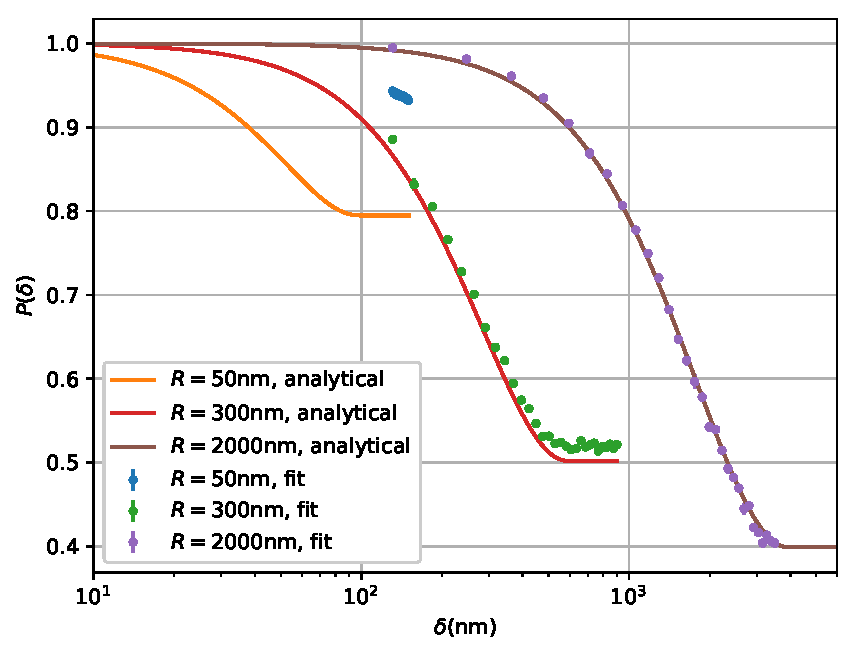
\includegraphics[width=\textwidth]{simulation-plot-rms-ISO-8}
		\caption{ISO 8.}
		\label{fig:simulation-plot-rms-ISO-8}
	\end{subfigure}
	\caption{$P_{exp}(\delta)$ values derived using the RMS method together with analytical $P(\delta)$ curves for three different samples. The data is the same as shown in Figure \ref{fig:simulation-plot-gauss}.}
	\label{fig:simulation-plot-rms}
\end{figure}

\section{Discussion}
When comparing Figures \ref{fig:simulation-plot-gauss}, \ref{fig:simulation-plot-rms}, generally speaking both analysis methods give similar results. The RMS method seems to be more consistent, better matching $P(\delta)$ for $R=\SI{2}{\micro\meter}$ in Figure \ref{fig:simulation-plot-rms-FOIL-4.321} as compared to \ref{fig:simulation-plot-gauss-FOIL-4.321}, with the Gaussian fit making an error there. The loss of polarization for $\lambda$ other than $\lambda_0$ in the foil flippers \cite{kraan2003} could perhaps explain this error, as this causes the modulation spectrum to differ from what is expected. Using RMS also gives a more reasonable fit of the $R=\SI{50}{\nano\meter}$ sample by appearing to capture some of the curvature of $P(\delta)$ in Figures \ref{fig:simulation-plot-rms-FOIL-4.321}, \ref{fig:simulation-plot-rms-WSP-4.321}, \ref{fig:simulation-plot-rms-ISO-4.321}. Although corrections compensating for a too-low detector $Q$-range \cite{kusmin2017} were not performed, it could be that the corrected analytical $P(\delta)$ curve for this sample looks somewhat like the $P_{exp}(\delta)$ fitted to data. Both methods also give a $P_{exp}(\delta)$ for $R = \SI{300}{\nano\meter}$ that is shifted upwards compared to the expected $P(\delta)$ for all instruments with $\lambda_0 = \SI{8}{\angstrom}$, indicating that $P_{exp}(\delta)$ probably accurately describes the fitted $y$-range of $V(y)$ data but cannot simply be said to estimate $P(\delta)$. Fitting only the middle $\SI{2}{\milli\meter}$ instead of the middle $\SI{6}{\milli\meter}$ of the detector reduces this error somewhat but not entirely. This can perhaps be explained by the relatively high $\tau = 0.6893$ as listed in Table \ref{tab:sample-thickness}, causing a relatively high degree of multiple scattering and a larger fraction of scattered neutrons to go undetected making $P_{exp}(\delta)$ a poor estimate of $P(\delta)$. Another reason could be the greater $\Delta\lambda$ of designs at $\lambda_0 = \SI{8}{\angstrom}$, causing errors of the type discussed in Section \ref{c3.6}. Additionally, the greater spread in scattering angles could play a role as $Q\propto 1/\lambda$, making the same $Q$ scatter into larger angles for the colder $\lambda$ values in the spectrum. This would also reduce the quality of estimate $P_{exp}(\delta)$ and the effective $Q$-range of the instrument.

This could mean that instruments with $\Delta\lambda/\lambda_0 = 0.1$ or similar like the three presented here with $\lambda_0 = \SI{8}{\angstrom}$ are more restricted for lower values of $\delta$ than predicted using the constraint model presented in Chapter \ref{c4:constraints}, meaning that measuring wide $\delta$ ranges might be harder when using colder wavelengths available at a $T=\SI{20}{\kelvin}$ using a velocity selector. 

An alternative explanation would be that $P(\delta)$ should be corrected for the spread in $\lambda$ as discussed in Section \ref{c3.6}. This would also explain why the monochromatic $P(\delta)$ expression describes the fitted $P_{exp}(\delta)$ values well when $\Delta\lambda/\lambda_0 = 0.01$ but not when $\Delta\lambda/\lambda_0 = 0.1$. It is not clear what such a correction would look like. An alternative would be to use Fourier methods, but as indicated in Section \ref{c3.6} this can be complicated by frequency resolution constraints.